\section{Circuit with NPN and PNP bipolar junction transistors}
Give the circuit in Figure \ref{lab3_ex7_de}. Calculate the Voltage at all nodes and the current in all branches.
Assume the current gain of both transistors is the same at $\beta$ = 100. Then perform a simulation and compare the result with the theoretical calculation.

\begin{figure}[h]
    \centering
    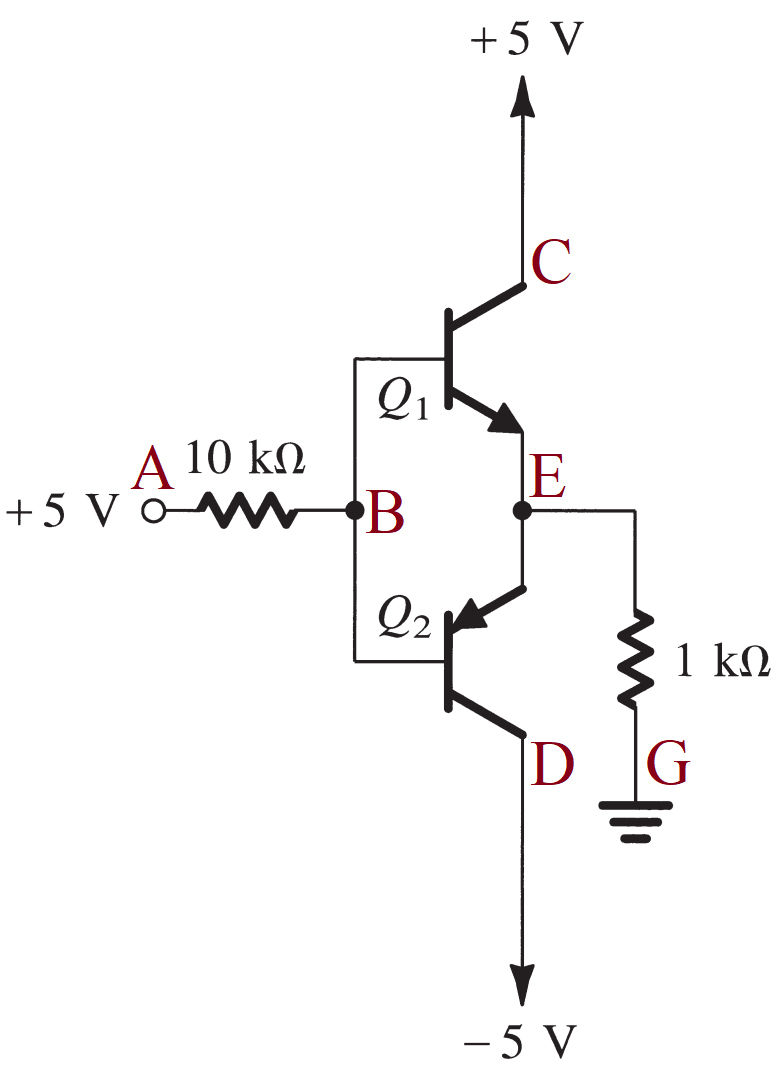
\includegraphics[width=6cm]{graphics/ex7/lab3_ex7_de.png}
    \caption{Circuit with NPN and PNP bipolar junction transistors}
    \label{lab3_ex7_de}
\end{figure}

\subsection{Theoretical calculation}
Note:

Explanations, formulas, and equations are expected rather than only results.

Ta có $V_E < V_B$ nên transistor $Q_2$ là cut off

Theo KVL, KCL, định luật Ohm, ta có các phương trình sau:
\[
I_{BE} \, (\text{hereinafter called } I_B) = \frac{V_A - V_{BE} - 1000 (\beta +1)I_B}{10000} \quad (1)
\]
Giải (1), ta có:
\[
I_B = \frac{V_A - V_{BE}}{11000 + 1000 \cdot \beta}
\]
\begin{align*}
    I_C &= \beta \cdot I_B\\
    I_{EG} &= I_E = (\beta + 1) \cdot I_B\\
    V_E &= 1000 \cdot I_E\\
    V_B &= V_A - 10000 \cdot I_B\\    
\end{align*}

\subsection{Simulation}
Your image goes here

\begin{figure}[h]
    \centering
    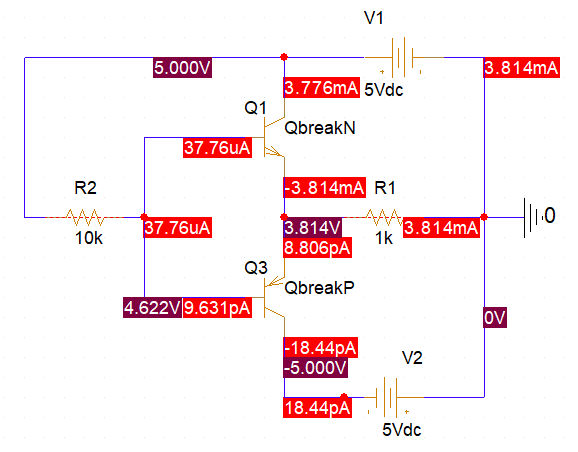
\includegraphics[width=0.7\textwidth]{graphics/ex7/f1.PNG}    
\end{figure}

\subsection{Comparison}
% $I_B$ (In theory) =  $I_B$ (simulation) = 37,76 $$

% $I_C$ (In theory) =  $I_C$ (simulation) = 

% $I_{EG}$ (In theory) =  $I_{EG}$ (simulation) = 

% $V_E$ (In theory) =  $V_E$ (simulation) = 

% $V_B$ (In theory) =  $V_B$ (simulation) = 

\[
I_B \, (\text{In theory}) = 38.7 \, \mu \text{A} \quad I_B \, (\text{simulation}) = 37.76 \, \mu \text{A}
\]
\[
I_C \, (\text{In theory}) = 3.87 \, \text{mA} \quad I_C \, (\text{simulation}) = 3.776 \, \text{mA}
\]
\[
I_{EG} \, (\text{In theory}) = 3.91 \, \text{mA} \quad I_{EG} \, (\text{simulation}) = 3.814 \, \text{mA}
\]
\[
V_E \, (\text{In theory}) = 3.91 \, \text{V} \quad V_E \, (\text{simulation}) = 3.814 \, \text{V}
\]
\[
V_B \, (\text{In theory}) = 4.613 \, \text{V} \quad V_B \, (\text{simulation}) = 4.622 \, \text{V}
\]
